%%%%%%%%%%%%%%%%%%%%%%%%%%%%%%%%%%%%%%%%%%%%%%%%%%%%%%%%%%%%%%%%%%%%%%%%%%%%%%%
%                         File: osa-revtex4-1.tex                             %
%                        Date: April 15, 2013                                 %
%                                                                             %
%                              BETA VERSION!                                  %
%                   JOSA A, JOSA B, Applied Optics, Optics Letters            %
%                                                                             %
%            This file requires the substyle file osajnl4-1.rtx,              %
%                   running under REVTeX 4.1 and LaTeX 2e                     %
%                                                                             %
%                   USE THE FOLLOWING REVTeX 4-1 OPTIONS:                     %
% \documentclass[osajnl,twocolumn,showpacs,superscriptaddress,10pt]{revtex4-1}%
%                    %% Use 11pt for Applied Optics                           %
%                                                                             %
%               (c) 2013 The Optical Society of America                       %
%                                                                             %
%%%%%%%%%%%%%%%%%%%%%%%%%%%%%%%%%%%%%%%%%%%%%%%%%%%%%%%%%%%%%%%%%%%%%%%%%%%%%%%

%\documentclass[osajnl,twocolumn,showpacs,superscriptaddress,10pt]{revtex4-1} %% use 11pt for Applied Optics
\documentclass[osajnl,preprint,showpacs,superscriptaddress,12pt]{revtex4-1} %% use 12pt for preprint option
\usepackage{amsmath,amssymb,graphicx}
\usepackage{multirow}
\usepackage{setspace}
\usepackage{caption}
\usepackage{subcaption}
%\usepackage{longtable}

%\usepackage{draftwatermark}
%\SetWatermarkText{DRAFT}
%\SetWatermarkScale{6}


\newcommand{\procspie}{{Proc. ~SPIE}}
\begin{document}

\title{Optical characterization of gaps in directly bonded Si compound optics using infrared spectroscopy}

\author{Michael Gully-Santiago}\email{gully@astro.as.utexas.edu}
\author{Daniel T. Jaffe}
\affiliation{Department of Astronomy, The University of Texas at Austin, Austin, TX, 78712, USA}

\author{Victor White}
\affiliation{NASA Jet Propulsion Laboratory, Pasadena, CA}


\begin{abstract}
Silicon direct bonding offers flexibility in the design and development of Si optics by allowing manufacturers to combine subcomponents with a potentially lossless and mechanically stable interface. The bonding process presents challenges in meeting the requirements for optical performance because air gaps at the Si interface cause large Fresnel reflections. Even small (35 nm) gaps reduce transmission through a direct bonded Si compound optic by 5\% at $\lambda = 1.15 \; \mu$m at normal incidence. Understanding the optical effects of such gaps and evaluation of various methods for preventing or eliminating them demands that we have a method for measuring not only the two-dimensional extent of the gaps but also their axial extent.  Existing methods for studying gaps provide only poor measures of this axial extent.  We describe a bond inspection method that makes use of precision transmission spectroscopy.  Using spectroscopy, we can detect and measure gaps as small as 8 nm by measuring transmission as a function of wavelength. Our approach involves modeling multiple incoherent reflections within the substrate interfaces with a wave transfer matrix, modified for intensities rather than complex amplitudes. We describe the measurement and analysis techniques and demonstrate the validity of the approach by measuring bond gaps of known depths produced by microlithography.
\end{abstract}

\ocis{(030.1670) Coherent optical effects; (050.2230) Fabry-Perot; (120.2230)   Fabry-Perot; (120.2830) Height measurements; (120.4610) Optical fabrication; (120.7000) Transmission; (120.7000)   Transmission; (220.4840) Testing; (230.4170) Multilayers; (240.1485) Buried interfaces;  (300.6340) Spectroscopy, infrared; (310.6628)  Subwavelength structures, nanostructures}

\maketitle %% required

\section{Introduction}

\subsection{Why Silicon is good}
Crystalline silicon is an excellent optical material for the infrared. Si has a high refractive index ($\sim$3.4, \cite{2006SPIE.6273E..77F}) and superb transmission from slightly longer than the equivalent wavelength of its band gap ($\sim$1.15 $\mu$m) to about 6.5 $\mu$m \cite{PhysRev.108.268, PhysRev.78.178} and in the far-IR \cite{doi:10.1117/12.323764}.  It has adequate transmission  ($\alpha \sim 1$ cm$^{-1}$) for many purposes in the 18-30 $\mu$m region as well \cite{doi:10.1117/12.323764}.  There is an extensive industrial infrastructure for the production of ultrapure Si and for polishing and lithographic patterning and etching of optical parts.  

\subsection{Why bonding is good and AR Coating is bad}
As with a number of glasses and crystalline optical materials, it is possible to form strong physical bonds between two planar or conformal silicon surfaces.  One advantage of this direct Si-Si bonding of macroscopic optical parts is that it facilitates the manufacture of complex optical subsystems, for example double-convex aspheres, combinations of lenses, prisms, and transmission gratings, and pairs of gratings oriented at right angles \cite{2012SPIE.8450E..2TV, 2010SPIE.7739E.123G}.  A second important advantage is that a sufficiently close bond is optically lossless, an important consideration not only for its effect on throughput but also because it can eliminate concerns about optical ghosts.  The remaining advantages of bonding stem from various difficulties encountered in antireflection coating a high index material in the near and mid-infrared:  There is a limited choice of index-matching materials, in particular at longer wavelengths.  Systems often are used at cryogenic temperatures and considerations of differential thermal expansion, brittleness and hygroscopic properties can restrict the choice of coatings even further. It is hard to get good antireflection performance across broad spectral ranges and at a range of incidence angles. 

\subsection{Silicon Bonds- history and techniques}

There are several good reviews of Si bonding that include accounts of the history of the field and a description of process alternatives, metrology, and problems \cite{1998AnRMS..28..215G,Masteika2014}.  The foundation paper on Si bonding came in 1986 \cite{1986JAP....60.2987S}. After that, there was a sequence of papers that used IR imaging to look for evidence of defects in the bond. Stengl et al. (1988) and Goesele et al. (1995) \cite{1988JaJAP..27L2364S, 1995ApPhL..67.3614G} directly monitored the bond propagation with IR imaging. Lehman et al. 1989 and Goesele et al. \cite{1989JaJAP..28L2141L, 1995ApPhL..67.3614G} demonstrated gap-free bonding in a micro- cleanroom, in which the bonding process occurs immediately after a rinse-spin-vacuum cycle inside of a vacuum enclosure.  Other authors investigated the growth of bubbles at bond interfaces with time and the elimination of some or all of these bubbles after annealing bonded parts at temperatures of 800-1100 $^\circ$C \cite{Horn2009, Masteika2014}.

The chemistry of the bonding interface began to be understood with infrared absorption spectroscopy and multiple internal reflection spectroscopy\cite{feijoo1994}, which lent credibility to the idea of distinct temperature phases and evidence for Si$-$H bonds\cite{1995ApPhA..61..101R}.  These results ultimately helped to flesh out a robust picture of the chemistry as a function of anneal temperature\cite{1996JaJAP..35.2102R, 1998AnRMS..28..215G}.  Other variables potentially affecting bond strength were studied, for example surface roughness\cite{JJAP.37.4197}, surface topography \cite{2001JOptA...3...85G}, surface preparation\cite{1996ApPhL..68.2222T}, annealing time \cite{2000JAP....88.4404H}, ambient pressure and substrate thickness \cite{1995ApPhL..67..863G, 2007ApOpt..46.6793H}, and moisture and defects \cite{2001JAP....89.6013L}.  Notably, \cite{JJAP.37.4197} found that surface roughness above 1.3 nm RMS results in poor bonding quality in their sample of wafers etched with Argon.  Results from studies of surface topography are inconclusive\cite{2001JOptA...3...85G}.

\subsection{Requirement:  Do better than coatings averaged over the surface}

If Si-Si bonds are to be a useful part of the optical designer's toolbox, the bonds must have transmission losses similar to or lower than the concatenated losses of two antireflection coated surfaces over the operating wavelength (typically $< 4$\%).  For Si-air gaps, where the full Fresnel loss is $\sim30\%$ per interface this requirement translates to physical gaps or bubbles having an axial extent of $ < 35\;$nm.  If the optical layout does not eliminate pupil ghosts from the flat Si surfaces, there are additional requirements on the reflectivity of individual bubbles in the bond. While completely bonded Si parts will be completely lossless at the interface, problems on different scales with different physical origins can lead to less-than-perfect bonds.  On the smallest scales, imperfect cleaning can leave small voids where particulates hold the bonding planes apart or where hydrocarbons can serve as catalysts for gap formation.  Even in the best of cleanrooms, particles at the optically significant 10-20 nm scale can be present in relatively high abundance. Figure 5 of Cooper 1986\cite{doi:10.1080/02786828608959094} shows the surface flux (particles cm$^2$ s$^{-1}$) vs. particle size ($\mu$m). There will be roughly $10^4$ times more 10 nm sized particles than 1 $\mu$m sized particles.  On larger scale, gaseous hydrogen, which is a byproduct of the hydrophilic bonding process, can migrate into the bond and form local bubbles \cite{Masteika2014}.  Most of the bonding literature concerns itself with wafer bonding.  In bonding wafers to each other or to thicker optically polished Si disks, one or both of the partners can conform as the bonding front propagates.  In optics, however, both of the bonding partners will likely be thicker and more mechanically rigid.  When bonding two thick substrates, differences in the shapes of the polished surfaces can potentially lead to topological inconsistencies that prohibit some areas from bonding.

\subsection{Existing detection schemes}
Verification that an optical bond meets its requirements and diagnosis of possible problems in the bonding technique require an accurate assessment of the geometry and lateral and axial dimensions of any defects.  Since silicon is opaque in the optical, the most straightforward technique for detecting defects in the bond is to image it in the infrared.  Fresnel losses will cause unbonded regions to appear darker than regions where the bond is perfect.  In cases where the axial extent of the gap is a wavelength or more, Newton rings appear in the image of the gap.  X-ray topography \cite{Mitani1990} exploits the change in optical density along lines of sight to allow precise high spatial resolution measurements of the spatial extent of gaps with axial dimensions as small as a few nanometers but not of the axial extent itself. In ultrasound microscopy, the density change at the gap interface produces reflections of sound waves and enables mapping the lateral gap dimensions but also produces only limited information about the axial dimension \cite{2000RScI...71.1869G}.

\subsection{Technique}
We describe here a new technique for measuring the axial extent of small gaps, founded upon the ability to measure transmission as a function of wavelength with high accuracy.   A recent generation of stock near-infrared spectrophotometers like the Cary5000 from Agilent offer 0.2\% precision and good repeatability.  We use the wavelength dependence of the transmission and a model of the gap as a closely-spaced Fabry-Perot to measure axial gaps down to a few tens of nanometers in size.  In order to verify the applicability and accuracy of the technique, we have used microlithography to create small artificial gaps of known size in wafers that we then bond and measure.

\subsection{What level do you need to measure to}
For all types of gaps and bubbles, our technique needs to provide an accurate assessment of the transmission loss at the operating wavelength.  For finite-sized bubbles, measurement of the axial dimension helps us to assess the effects of high-temperature annealing \cite{Horn2009, Masteika2014} on removal of hydrogen bubbles.  A wavelength-dependent transmission variation can also indicate the presence of large numbers of gaps that are too small to resolve spatially, as one might expect if there are many very small contaminants present along the interface.  Our technique must be able to characterize gaps with losses of a few percent at the operating wavelength.  A 2\% loss at 1.15 $\mu$m corresponds to a gap of XX nm at normal incidence and the gap size for a loss of this magnitude scales linearly with wavelength.  We therefore need to be able to measure transmission as a function of wavelength to a fraction of a percent, including all systematic errors, for devices operating near 1 $\mu$m and to a somewhat looser standard for devices operating at longer wavelengths. 

\section{Conceivable pitfalls in Si-Si direct bonding}

It is conceivable that there are particles in between the Si interfaces.  Particle contaminants are discussed in \cite{Mitani1990}.

Another possible source of gaps at the bond is inherent roughness in the initial surfaces that leads to a failure to conform.  Stiff non-flat Si surfaces will not conform upon contact leaving the complement of the aberrations as an air gap. Unconventional thick ($\sim$ 30 mm) Si pucks are less conformal than wafers are, so we expect thick substrates could have gaps even in the absence of particles.  Most of our thick substrates are optically polished to less than 60 nm peak to valley over the 3 to 4 inch diameter clear aperture.  We assume that, if enough pressure is placed on the substrates during bonding, then the surfaces will come in contact and zipper up.  Subsequent annealing will strength the bond.

\section{Si$-$Si Fabry P\`{e}rot measurement theory}
\label{secTheory}

\subsection{The Si$-$Si interface gap is a low Finesse Fabry-P\`{e}rot etalon}

Our measurement technique exploits the large Fresnel reflection \cite{2001opt4.book.....H} at the Si$-$vacuum interface.  The refractive index of silicon at room temperature ranges from 3.55$-$3.45 from $\lambda = $ 1150$-$2500 nm \cite{2006SPIE.6273E..77F}, one of the largest refractive indices of any conventional material.  The Fresnel reflection is about 30\% per surface, much larger than the $4-7\%$ per surface of the many optical materials with refractive indices in the range $1.5-1.7$.  Figure \ref{figSiIndexFinesse} shows the refractive index as a function of wavelength for room temperature,  computed using the coefficients from \cite{2006SPIE.6273E..77F}.

\begin{figure}[htbp]
\centerline{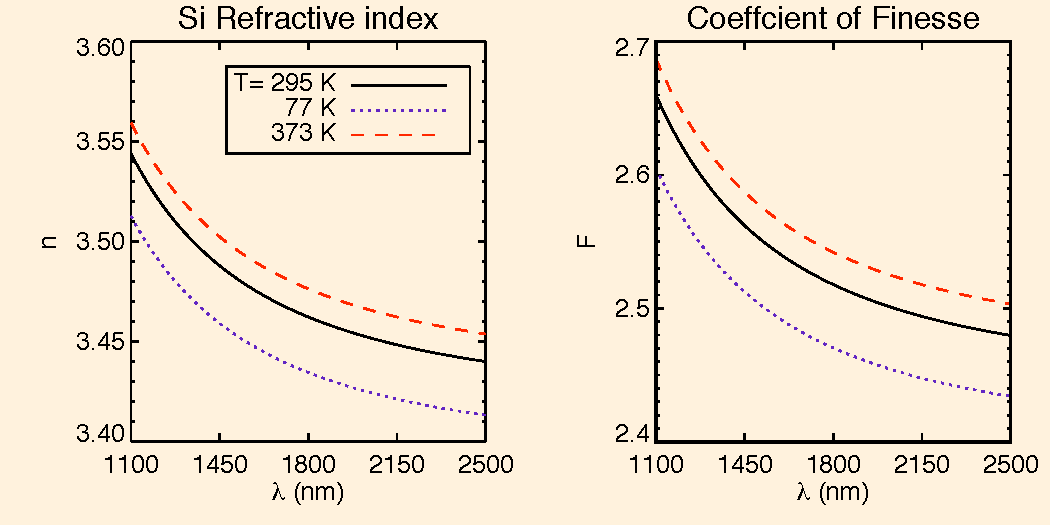
\includegraphics[width=0.95\columnwidth]{figs/SiIndexAOmgsFinesseFig.pdf}}
\caption{Plot of refractive index, $n$, and coefficient of finesse, $F$, as a function of wavelength, $\lambda$.\label{figSiIndexFinesse} We computed the temperature dependent refractive index from the tabulations of CITE\texttt{2006SPIE.6273E..77F}.  The coefficient of finesse is defined in Equation \ref{eq:FabPerot}.  We assume $T= 295\;$K for all calculations in this article.}
\end{figure}

We can treat a small Si$-$Si interface gap between two almost-bonded silicon parts as a low-Finesse Fabry-P\`{e}rot etalon\cite{2007fuph.book.....S}.  The key property of an etalon is that it has a cavity enclosed between two smooth and parallel reflective surfaces where the requirements for smoothness and parallelism depend on the reflective finesse of the cavity.  For the narrow air gaps we consider here and for the modest reflectivity of a Si-vacuum interface, most gaps at Si-Si bonds will form effective etalons over most of their area.  The transmission through a Fabry-P\`{e}rot depends on the wavelength of light, the reflectivity of the etalon sidewalls, and the size of the gap.  We assume transmission is at normal incidence, the refractive index of the gap is 1.0, and the material is at $T= 295\;$K.  We compute the reflectivity for an Si$-$vacuum interface, which is a modest function of wavelength through the refractive index of Silicon, $n(\lambda, T)$ \cite{2006SPIE.6273E..77F}, as shown in Figure \ref{figSiIndexFinesse}.  We drop the subscripts on the refractive index $n(\lambda, T) \rightarrow n$ and the coefficient of finesse $F(\lambda, T) \rightarrow F$ for clarity.  The computation is simply Fresnel's law at normal incidence:

\begin{eqnarray}
R = \frac{(n-1)^2}{(n+1)^2} \label{Eq:FresnelR}\\
F \equiv \frac{4R}{(1-R)^2} \label{Eq:coeffF}
\end{eqnarray}

We define the coefficient of finesse\cite{2007fuph.book.....S}, $F$ (Equation \ref{Eq:coeffF}), in the customary way to encapsulate the Fabry-P\`{e}rot etalon's dependence on reflectivity.  The right panel of Figure \ref{figSiIndexFinesse} shows the coefficient of finesse as a function of wavelength for $T = 295\;$K and $T = 77\;$K.  Si absorbs negligibly longward of $\lambda$ = 1250 nm, which we verified by comparing the transmission of Si reference samples of different thicknesses (Figure \ref{figSiAbsorbfig}).  We measured the ratio of transmissions of a 0.5 mm thick double side polished Si wafer and a 3.0 mm Si puck.  Figure \ref{figSiAbsorbfig} verifies a key assumption that we make when comparing the transmission of scrap Si of different provenance and thickness.  Specifically, double side polished 3 mm thick Si pucks and 0.5 mm thick Si wafers have indistinguishable transmission at the $<0.2$\% level longward of 1250 nm.  The Si refractive index is indistinguishable from sample to sample for the wavelength ranges we care about- the non-absorbing wavelengths greater than about 1250 nm.  \cite{2006SPIE.6273E..77F} cites the wide variety of values for refractive index from the literature as evidence that batch-specific Si should be used as a reference for cases in which absolute accuracy greater than $\pm5\times10^{-3}$ is desired.  An absolute deviation of $\pm5\times10^{-3}$ in refractive index corresponds to a Fresnel transmission difference of about 0.2\%, which is comparable to our measurement uncertainty.  In the next subsection we work out the wavelength dependent transmission for the air etalon.

\begin{figure}[htbp]
\centerline{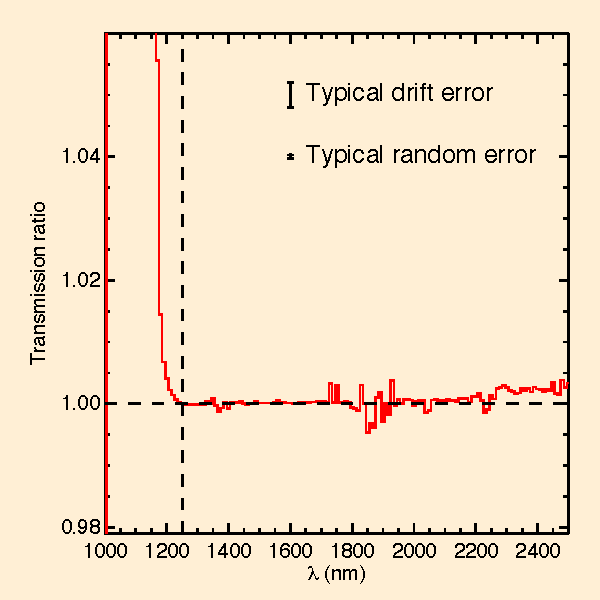
\includegraphics[width=0.40\columnwidth]{figs/fpAbsorbfig_alt}}
\caption{Ratio of transmission of a 0.5 mm thick Si wafer to that of a 3.0 mm thick Si puck.  \label{figSiAbsorbfig} We detect Si absorption shortward of $\lambda$ = 1250 nm.  The individual measurements have correlated uncertainties attributable to lamp drift at the level of 0.2\%.  The random uncertainties are typically about 0.02\% per sample, though some wavelength regions (e.g. 1700-1900 nm) demonstrate much greater per sample uncertainties.  Absorption longward of 1250 nm (vertical dashed line) is negligible.}
\end{figure}

\subsection{Predicted transmission spectrum for bonded Si with finite interface gap}
\label{secTheory}
A pair of bonded silicon wafers or pucks with a small gap actually forms three coupled cavities with the air gap as the the central cavity.  The outer cavities, those within the Si, however, were not produced with coherence in mind.  Their sides are not necessarily flat and parallel to the required level and the specifics of their deviation from perfect etalons are usually not known to the level necessary to treat them as coherent structures in the analysis.  The multiple internal reflections within the Si therefore present a hurdle to an analysis of the air gaps whereas the gap size is small enough that the cavity it forms can always be treated as a coherent structure.  Treatments for multiple coherent reflections have been described in detail in the optics literature \cite{2007fuph.book.....S}.  The wave transfer matrix technique treats each dielectric interface as a matrix with elements relating the pre- and post- interface complex amplitudes in the left and right directions.  We adapted the wave transfer technique for incoherent interactions \cite{2002ApOpt..41.3978K} to deal with the cavities within the thick Si substrates.  Specifically we constructed an incoherent wave transfer matrix whose elements relate the intensities (and not complex amplitudes) before and after an interface.  The details appear in Appendix \ref{sec:Append-IMRTMM}.  We computed the transmission for two scenarios: first a double side polished (DSP) Si sample with no gap, and second a pair of bonded Si samples with a gap thickness $d$.  The DSP Si sample with no air gap has a transmission equal to:

\begin{eqnarray}
T_{DSP} = \frac{2n}{1+n^2} \label{eqnAbsDSPtrans}
\end{eqnarray}

which has an average value of about 53\%.  Note that this transmission is above a na\"ive value of $T_{DSP}=(1-R^2)$, which does not take into account multiple incoherent reflections, and is therefore an underestimate.  Figure \ref{figAbsoluteTrans} shows a plot of Equation \ref{eqnAbsDSPtrans} in the wavelength range $1200-2500\;$nm.  If the Si wafer path thickness is less than the coherence length for the given spectral bandwidth, then our assumptions break down and the multiple reflections would interfere coherently, and the Si wafer would behave as a Fabry-P\`erot etalon.  We do not treat this case here since our focus is on thick substrates with small gaps between the interfaces.


\begin{figure}[htbp]
\centerline{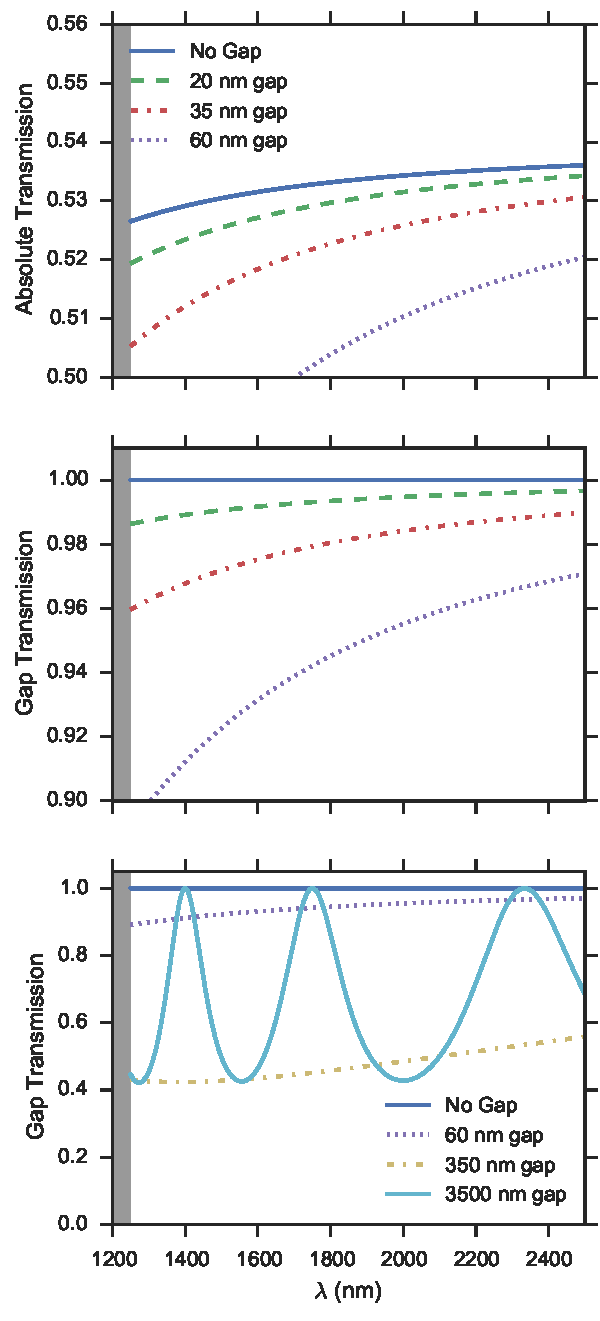
\includegraphics[width=0.40\columnwidth]{figs/etalon_trans.pdf}}
\caption{\label{figAbsoluteTrans}The family of normal-incidence curves for transmission as a function of wavelength for various gap sizes in bonded Si optics.  \emph{Top panel}: Absolute transmission through a Si substrate with no gap (top denim-blue solid curve), and small gaps of axial extent 20 nm (green dashed curve), 35 nm (red dash-dotted curve), and 60 nm (purple dotted curve).  The absolute transmission through Si depends on wavelength since the refractive index depends minutely on wavelength.  The curves assume that multiple reflections within the Si substrates add incoherently as discussed in detail in Appendix \ref{sec:Append-IMRTMM}.  \emph{Middle panel}: The ``Gap Transmission'', defined as the Absolute transmission through a sample normalized by the absolute transmission through a gapless sample. The gap sizes and colors are the same as in the top panel.  \emph{Bottom panel}: ``Gap Transmission'' for larger gaps, spanning 0-3500 nm.  The 3500 nm sized gap (cyan solid line), demonstrates characteristic Fabry-P\`erot etalon fringes.}
\end{figure}

Consider a pair of bonded Si samples with a gap thickness $d$. We derive the absolute transmission of bonded Si substrates with a gap in Equation \ref{eqn:Tetalon} in the Appendix.  We normalize the absolute transmission by the transmission with no gap to isolate the effect of the gap.  We call this normalized transmission the etalon transmission $T_{e}$.

\begin{eqnarray}
T_{e} = \frac{n^2+1}{2 n F \sin ^2(2\pi \frac{d}{\lambda})+n^2+1} \label{eqFP}
\end{eqnarray}

In the limit $\lim_{d \to 0} T_e \rightarrow T_{DSP} $ and the etalon approaches 100\% transmission.  Figure \ref{figAbsoluteTrans} shows a plot of Equation \ref{eqFP} for gap sizes, $d$, of 0, 20, 35, 60, 350, and 3500 nm.  The bottom two panels show the ``gap'' transmission, the value of the throughput with the losses from the outer Si cavities divided out.  For the very largest gap, large fringes appear as the cavity resonance of the air gap modulates the transmission.  Below a $\lambda/2$ gap size the effect of the gap manifests itself as a wavelength-dependent diminution of the transmission.  For the smallest $35-60$ nm gaps, there is a $2-6\%$ decrease in gap transmission from $2400\;$nm down to $1250\;$nm.  It is the magnitude and wavelength dependence of this transmission spectrum that provides information about the axial extent of the gap.

\section{Laboratory demonstration: Embedding gaps of known sizes}

We evaluated our metrology method by embedding gaps of known sizes in the interface and measuring the effects of these gaps on IR transmission.  The substrate thicknesses ranged from 0.5 to 3.3 mm.  We denote substrates with thicknesses larger than 1 mm as ``pucks'' and substrates with thickness less than 1.0 mm thick as ``wafers''.  We distinguish the two classes of substrate thickness based on the anticipation that thin substrates will conform more easily to their bonding partner substrates.  There is also evidence that bond front propagation is slower in thick pucks \cite{2007ApOpt..46.6793H} than in wafers.  Our ultimate goal is to bond optics with thicknesses as large as 30 mm.

The three important characteristics of gaps are their axial extent, their lateral areal extent, and their areal fill factor.  To fabricate our test samples, we used photoresist lithography to pattern Si substrates, and we bored holes with inductively coupled plasma etching.  We used two different gases with low and high etch rates, CHF$_3$ on Si exhibited about 0.3 nm/second etch rate, SF$_6$ exhibited about 1 micron/minute.  Tables \ref{tabbondexper} and \ref{tblPatternFills} give information about the hole patterns and depths, as measured with Veeco NT9100 Optical Profiler for the small depth, and Dektak stylus profilometry for the large depth.

The fill factor is defined as the pattern area covered by gaps relative to the total pattern area.  In a second round of experiments, we achieved gap sizes of 14$-$95 nm on four substrates with three meshes with coarse, medium, and fine boxes, each with 50\% fill factors.  No attempt was made to verify the delivered fill factor, but since high precision lithographic processes were employed, we assign no uncertainty to the difference between the delivered fill factor and the designed fill factor.  For measurements taken with the Veeco NT9100 Optical Profiler, uncertainties were constructed by inspecting the histogram of topology, as shown in Figure \ref{figVS20pattern}.  The large-scale distortions were removed from the topology by masking and flattening to ensure that the uncertainties accurately reflect the distribution of measured heights.  The stylus profilometry measured values were simply assigned an uncertainty of 5\%, which was consistent with our intuition and experience.  Table \ref{tabbondexper} lists part numbers and descriptions for our bonded substrates.  

\begin{figure}[htbp]
\centerline{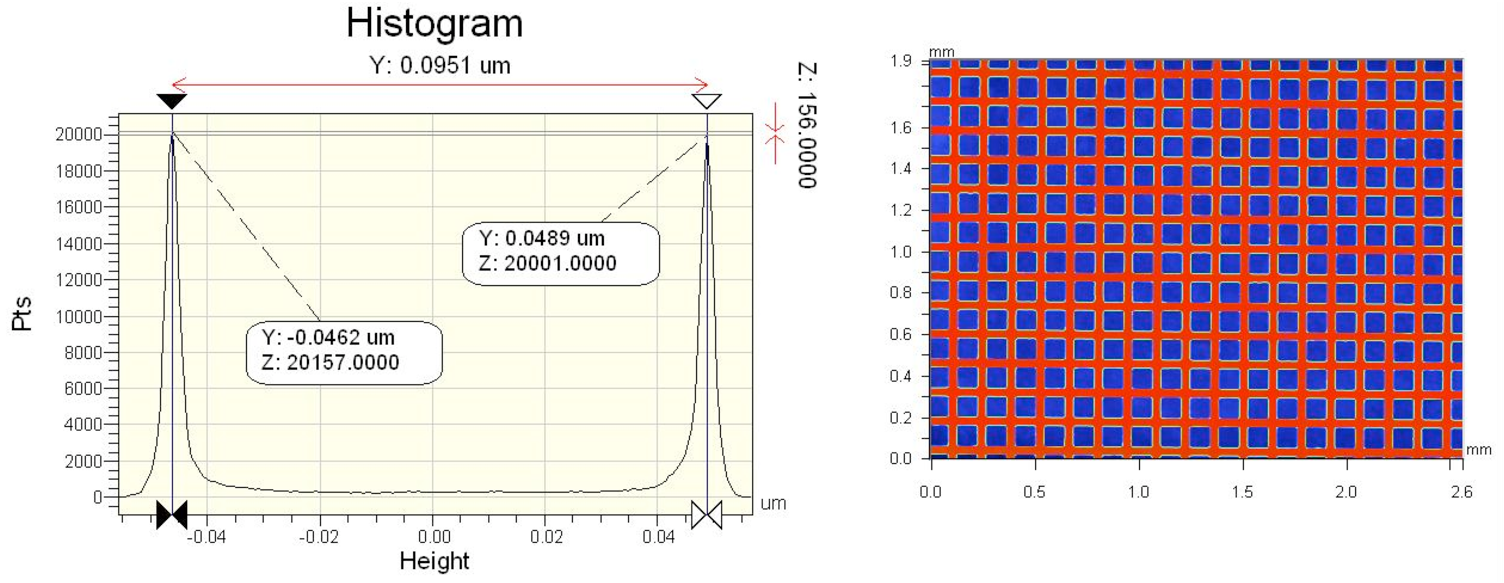
\includegraphics[width=1.0\columnwidth]{figs/VS20fineGapCrop.pdf}}
\caption{
\label{figVS20pattern}
Veeco optical profiler surface plot and histogram for part VS20-21 in the fine pattern section.  The 100 mm diameter VS20-21 is comprised of two thick silicon wafers.  We patterned three meshes with coarse, medium, and fine boxes, each with 50\% fill factors.  The depth was 95 $\pm$ 5 nm as indicated by the well-separated peaks in the Veeco profilometry histogram.  The fill factor for this and all mesh patterns was 50\%.  The purpose for these patterns was to have gaps of known axial extent against which we could test the optical metrology technique we describe in this article.}
\end{figure}

\begin{table}[h!]
\caption{UTexas Si bonding experiments \label{tabbondexper}}
\begin{center}
    \begin{tabular}{ c c c c c c}
    \hline
    Name & Diameter & Thickness & Pattern Type & Pattern Depth & Notes \\ 
    -  & mm & mm & - & nm & - \\
        \hline
    HA1     & 75   & 10 $\times$ 2& None & - & \\
    VG01   & 100 & 1 $\times$ 2 & None  & - &  \\
    VG02   & 100 & 3.3 $\times$ 2 &  None  & - &  \\
    VG03   & 100 & 3.3 $\times$ 2 &  Hole \&Petal & 4000$\pm$200 & \\
    VG04   & 100 & 1 $\times$ 2 &  Patchwork Islands & 15$\pm7$ & \\
    VG07   & 100 & 1 $\times$ 2 &  mesh C, M, F & 12$\pm7$ & \\ %see email from Victor on 5/16/13
    VG08   & 100 & 1 $\times$ 2 &  mesh C, M, F & 12$\pm7$ & \\
    VG09-12   & 75   & 1 $\times$ 2 & mesh C & 49 $\pm$6 & \\
    VG15-13   & 100 & 0.8 $\times$ 2 &  mesh C, M, F  &14 $\pm$2 & \\
    VS20-21   & 100 & 0.8 $\times$ 2 &  mesh C, M, F & 95 $\pm$5 & \\
    \hline
    \end{tabular}
\end{center}
\end{table}

\begin{table}[h!]
\caption{Patterned gap properties \label{tabPatternFills}}
\begin{center}
    \begin{tabular}{ c c c c }
    \hline
    Pattern & $f$ & feature size & bulk description \\ 
    - & \% & $\mu$m & - \\ 
    \hline
    Hole   & 100     &  -         & 25 mm diameter hole \\     
    Petal  & $\sim5$ & $\sim$2000 & 2 mm wide lines \\         
    Mesh F & 50      &         40 & 100 $\mu$m square holes, Fig. \ref{figVS20pattern}\\ 
    Mesh M & 50      & 200        & 500 $\mu$m square holes\\ 
    Mesh C & 50      & 620        & 1500 $\mu$m square holes\\     
        \hline
    \end{tabular}
\end{center}
\end{table}

We cleaned the surfaces before bonding to minimize the interfacial particle density.  The surface roughness was typically about 2 nm, as measured with a Veeco NT9100 Optical Profiler.  We measured the large scale surface flatness of the pucks.  The Fisba2 interferometer used for these measurements has a 50 mm diameter beam at $\lambda=$632.8 nm.  We found a typical peak to valley surface flatness of 2 waves over the central 50 mm diameter.  We prepared the substrates with standard cleaning procedures of solvents in a megasonic.  We then applied MHz frequency oxygen plasma ashing.  We soaked the wafers in DI water then dried with N$_2$.  We pressed the Si substrates together from the center to the outside.


\section{Measurement technique and correlated measurement errors}
\label{sec_aboutErrors}
We took transmission spectra of bonded Si wafers and pucks, and double side polished Si reference wafers using an Agilent Cary 5000 UV-Vis-NIR spectrophotometer.  Table \ref{tabCary5000pars} lists the typical measurement settings and tool performance.  The tool has a double monochromator, which reduces scattered light.  The vendor reported linearity exceeds 40 dB.

The Cary 5000 has four operation modes: single front, single back, double, and double reverse.  We experimented with single front and double modes.  Double mode takes a reference spectrum simultaneously with the target spectrum.  In both single and double mode, a baseline scan is taken with no sample in the measurement holder.  We automatically divide sample spectra by the baseline spectrum.  In single beam mode, the baseline measurements must be repeated about every half hour for post-process division.  In double beam mode the front beam is automatically divided by the rear beam, which corrects out lamp luminosity drift, for example.  

We estimated the uncertainty and measurement repeatability of single and double modes in the following way: we computed the RMS error and measurement repeatability in a single measurement by computing the standard deviation of a spectrum taken immediately after a baseline scan with no sample present.  We found that the mean value in single mode drifted by about 0.2\% over several measurements.  The standard deviation of the featureless spectrum was typically 0.02\% from point to point, with some portions of the spectrum demonstrating increased variance, perhaps attributable to atmospheric absorption.  In double beam mode, the spectrograph drift was much lower.  The simultaneous reference in double beam mode divides out the 0.2\% drift in the mean transmission level attributable to lamp drift that we saw in single beam measurements.  In double beam mode, the drift in mean transmission level is 0.02\%.  These values are accurate for measurements over a half hour timescale or less.  Table \ref{tabCary5000pars} summarizes the amplitudes of the drifts and individual measurement errors in both single and double beam modes.\emph{Correlated errors dominate the measurement uncertainty of our transmission spectra.}  The measurement uncertainty correlations are apparent in in Figure \ref{figSiAbsorbfig}.  In some parts of the spectrum, the mean drift is about ten times larger than the standard deviation of the spectrum.  Double beam mode has about ten times lower lamp drift but suffers from other instrumental artifacts, like disjointed spectra at the wavelengths of known grating changeover points.

The spectral sampling was ranged from 2.0 to 10.0 nm.  We used a spectral resolution of 5.0 nm.  We expect smoothly varying spectral features for all conceivable interface gaps in Si bonded wafers.  Specifically, Fabry-P\`erot fringes attributable to interfacial gaps in bonded Si will be well-sampled with 5 nm spectral resolution, so long as the interface gap is less than $\sim$100 $\mu$m.  The axial extents of such large gaps would be easily measurable by other means, like IR imaging.

\begin{table}[h!]
\caption{Summary of Cary 5000 measurement parameters \label{tabCary5000pars}}
\begin{center}
\begin{tabular}{ c c }
\hline
        Parameter (Units) & Value \\ 
\hline
        Spectral sampling interval (nm) & 2.0,10.0 \\
        Spectral resolution (nm) & 5 \\
        Typical measurement range (nm) & 1200-2500 \\
		Mean level drift uncertainty (\%) & 0.20 \\
		Random uncertainty (\%) & 0.02 \\
 		Beam size (mm $\times$ mm) & $2 \times 8$ \\
    \hline
    \end{tabular}
\end{center}
\end{table}


\subsection{IR bubble detection and limitations}

We looked for large gaps, detectable as ``IR bubbles'' \cite{1992JEMat..21..669M} with IR imaging.  The detector was an IR Vista $\alpha$NIR infrared focal plane array, with 312 $\times$ 252 pixels, with 30 $\mu$m square pixels.  We used a 50 mm F/2 lens, with a fiber optic white light illumination source.  The combination of the absorption of Si, the lamp spectrum and the detector responsivity led to an effective bandpass from approximately 1.15$-$1.6 $\mu$m.  The field of view was smaller than the 100 mm diameter wafers, so we dithered the sample.  Figure \ref{figVS2021_IR_image} shows an IR image of bonded sample VS20-21.  For this image, we coarsely flat-fielded the detector by observing a homogeneously illuminated white screen. Despite the flat-fielding, detector non-uniformities and vignetting are perceptible in our image as vertical stripes.  Mosaic-stitching errors are also perceptible.  It was easy to detect IR bubbles despite detector artifacts since the bubbles translate with the sample when we dither its position.  

We also used IR imaging to inspect VG09-12 and VG15-13.  We detected IR bubbles in all 3 of these bonded Si samples.  The observable bubble areal density varied from about 4 per 100 mm diameter bonded wafer pair to over 20 per bonded wafer pair.  The individual IR bubble diameters were as small as a few square millimeters up to 400 mm$^2$.  The IR bubbles had varied morphologies.  The structure within the IR bubbles was sometimes indicative of Newton's rings, exposing the presence of gaps larger than about $\lambda/2$ up to $\sim 15 \lambda$.  As expected, the unbonded DSP wafers show no such IR bubbles.  No attempt at quantitative measurement was made on the IR images due to evidence of a non-linear detector response.  The bulk morphologies were clear regardless of the detector response.  When IR imaging was available, it was leveraged to target IR specectroscopy in locations demonstrating presence or absense of IR bubbles, as desired.  In other cases when IR imaging was not available or ignored, spectra were taken at random positions on the wafer.

\begin{figure}[htbp]
\centerline{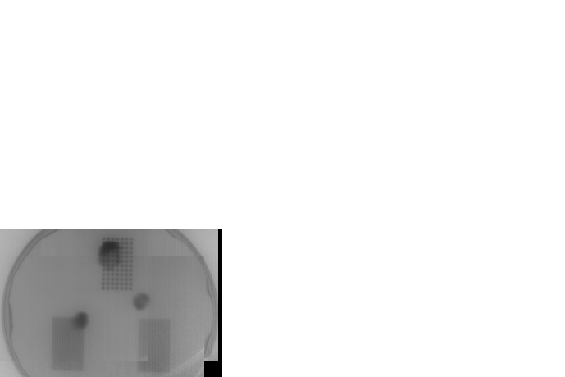
\includegraphics[width=0.4\columnwidth]{figs/VS2021_IR_image.pdf}}
\caption{
\label{figVS2021_IR_image}
IR image of part VS20-21. Three rectangular mesh areas are apparent (Table \ref{tabPatternFills}).  The coarsest mesh, C, shows substructure, while the medium and fine meshes are indistinguishable at the low resolution of the image.  The three dark spots are gaps at the interface of the direct bonded Si samples.}
\end{figure}


\section{Results of infrared spectroscopy of directly bonded Si}
\label{secResults}

The gaps in our test pairs should be a combination of the deliberately induced gaps and any inadvertent additional spaces caused by imperfections in the bonds.  We infer the axial extent of gaps in our samples with etched holes from their measured transmission spectra.  We use a Bayesian inference technique.  First we define a mixture model in which the observed normalized gap spectrum $T_{obs}$ is composed of a sum of a spectrum through a gap of axial extent $d$, and a spectrum through a perfect bond:

\begin{equation}
	T_{mix} = f T_{e} + (1-f) \label{eqnMix}
\end{equation}

where $f$ is the areal fill factor of the region exhibiting a finite gap size, and $1-f$ is therefore the areal fill factor of the perfectly bonded area.  $T_e$ is defined in equation \ref{eqn:Tetalon}.  The only free parameters in Equation \ref{eqnMix} are $d$ and $f$.  Both of these parameters are fixed in our direct bonded Si wafers with synthetic gaps, and are listed in Table \ref{tabPatternFills}.  These synthetic imbedded gaps therefore offer an excellent test of our ability to recover the gap axial extent $d$ and areal fill factor $f$ (Section \ref{secKnownGaps}).

Equipped with an observed spectrum and our mixture model, we constructed the Likelihood function \cite{2013sdmm.book.....I}.  The measurement errors are not assumed to be independent and identically distributed, and in fact are strongly correlated as discussed in Section \ref{sec_aboutErrors}.  To handle the correlated measurement errors we use Gaussian Processes \cite{rasmussen2006gaussian, DFMgp}.  The Gaussian Process takes into account the unknown but finite covariance structure by introducing a covariance matrix, $\boldsymbol{C}$ whose elements represent the correlations of each sample $i$ with every other sample $j$.  We parameterize the covariance matrix elements in the following way:

\begin{equation}
	C_{ij} = \sigma^2_{i}\delta_{ij}+a^2\exp{(-\frac{(\lambda_i-\lambda_j)^2}{2l^2})} \label{eqnGPkernel}
\end{equation}

where $\delta_{ij}$ is the Kronecker delta, and $\sigma_i$ are the independent measurement uncertainties on the $i^{\mathrm{th}}$ data point. We experimented with different values for $\sigma_i$.  When repeated DSP reference sample measurements were available, we estimated the $\sigma_i$ from the dispersion around mean-subtracted, detrended transmission spectra.  In other cases we simply adopted mean values from Table \ref{tabCary5000pars} for single and double beam modes respectively.  The latter assumption of homoscedasticity is fairly safe, since the correlated errors dominate in comparison to individual measurement errors.  The parameter $l$ controls the correlation length, and $a$ controls the amplitude of the noise.  We do not know $a$ nor $l$ and they are, in general, different for each measurement.  The value of $a$ should be close to the mean drift reported in Table \ref{tabCary5000pars}.  The value of $l$ could be small (tens of nm) to capture local variation attributable to atmospheric air absorption, or large (hundreds or thousands of nm) to capture global features attributable to lamp drift.  We allow both $a$ and $s$ to be free parameters in our fitting procedure.

We set our prior probability distribution functions \cite{2013sdmm.book.....I}, $\ln{p(d,f,a,s)}$ as uniform over a wide range of values for $\ln{a}$, $\ln{s}$, $d$, and $f$ consistent with visual inspection of each spectrum.  The final un-normalized posterior probability function, expressed as a natural logarithm is:

\begin{equation}
	\ln{p(d,f,a,s|\lambda, T_{obs}, \sigma)} \propto \ln{p(d,f,a,s)} -\frac{1}{2}\;\boldsymbol{r^\intercal}\boldsymbol{C^{-1}}\boldsymbol{r} -\frac{1}{2}\;\ln{\det{\boldsymbol{C}}} \label{eqnPosterior}
\end{equation}	

where the residual vector $\boldsymbol{r}$ is the data $T_{obs}$ minus the model $T_{mix}$.  We produce posterior samples with Markov Chain Monte Carlo (MCMC).  Specifically, we implemented \texttt{emcee}\footnote{https://github.com/dfm/emcee}\cite{emcee}, with 32 walkers, hundreds of burn-in samples, and 600-1000 iterations.  We initialized the walkers in the vicinity of our best guess for parameters based on visual inspection of the observed normalized Transmission spectra.  Figures \ref{figVG03full}, \ref{figVG03part}, and \ref{figVG12_corner} show examples of posterior samples including corner plots of the interesting physical parameters $d$ and $f$.

\subsection{Spectra of direct bonded Si with known gap sizes}
\label{secKnownGaps}

Figure \ref{figVG03full} shows a parameter determination for the measurement of a bond over a deep ($4000 \pm 200\;$nm) 100\% fill factor gap.  The analysis yields a best fit consistent with 100\% fill factor, and a depth of $3960 \pm 2\;$nm, well within the uncertainty of the physicsal measurement.  Figure \ref{figVG03part} shows a fit for a region of the same bonded pair where a nominally $4000\;$ nm deep, 2 mm wide trench crosses the field field scanned by the Cary 5000.  Analysis of this transmission curve gave a best fit depth of $4094 \pm 4\;$nm and a pattern fill factor of $4.6\% \pm 0.1\;\%$, both consistent with the part geometry.  These two results show that the formalism performs as expected on resonant gaps several wavelengths deep.  

In our test samples, the nominal gap we have induced in the sample represents a lower limit to the actual gap since poor adhesion of the non-continuous patterns may result in gaps larger than intended.  In this case, we modify our mixture model (Equation \ref{eqnMix}) to fix $f=0.5$ but allow two different gap depths:

\begin{equation}
	T_{mix} =  0.5 \times T_{e}(d_M + \epsilon) + 0.5 \times T_{e}(\epsilon) \label{eqnMix2Gaps}
\end{equation}

where the $d_M$ is the lab-measured mesh depth and $\epsilon$ is an undesired gap in excess of the mesh gap.  For $\epsilon =0$, Equation \ref{eqnMix2Gaps} reduces to Equation \ref{eqnMix} with $f=0.5$.  We capture the uncertainty in the lab-measured mesh depth by setting the prior on $d_M$ to a Normal distribution with standard deviation set by the values listed in Table \ref{tbl_experiments}.  

Figure \ref{figVG12} shows the results for a bonded pair with a 50\% fill factor mesh where the grooves in the mesh had a measured depth of $49\pm6\;$nm.  The apple green band shows the predicted range for the transmission curve.  The measurements lie below this band.  Figure \ref{figVG12_corner} demonstrates that $d_M$ and $\epsilon$ are degenerate, but consistent with a small $\sim 12\;$nm gap in excess of the mesh.  The presence of a number of bubbles both on and off the meshed areas of this and other samples (Figure \ref{figVS2021_IR_image}) lend credence to the idea that an additional gap of this magnitude was present at the position where we made the measurements but was not detected in the preparatory imaging.


\begin{table}[h!]
\caption{Inferred Gap sizes and fill factors \label{tbl_DerivedGapSizes}}
\begin{center}
    \begin{tabular}{ c c c c c }
    \hline
    Name & Region & Mode & $d$ & $f$ \\
    -  & - & S/D & nm & - \\
    \hline
    DSP & -    &   S  & $3^{+8}_{-2}$ & $0.260^{+0.456}_{-0.230}$\\
    VG09-12 & Off-Mesh    &   S  & $11^{+21}_{-7}$ & $0.25^{+0.46}_{-0.22}$\\
    VG03 & Hole    &   S  & $3960^{+2}_{-2}$ &  $0.999^{+0.001}_{-0.002}$\\
    VG03 & Petal   &   S  & $4094^{+4}_{-4}$ &  $0.046^{+0.001}_{-0.001}$\\
    \hline
    \end{tabular}
\end{center}
\end{table}

Figures \ref{figVG03full} to \ref{figVG12} show examples of the predicted and measured IR spectra.  Figure \ref{figVG03_f100} shows an example spectrum in which the measurement is consistent with the prediction for a gap with the known conditions.  Meanwhile, Figure \ref{figVG12_f50} shows a spectrum in which the measurement marginally exceeds the prediction (by about $\sim 3 \sigma$).  Other parts show less consistency with the prediction due to the difficulty of direct-bonding Si in the absence of thermal annealing.  

\begin{figure}[htbp]
        \centering
        \begin{subfigure}[b]{0.5\textwidth}
              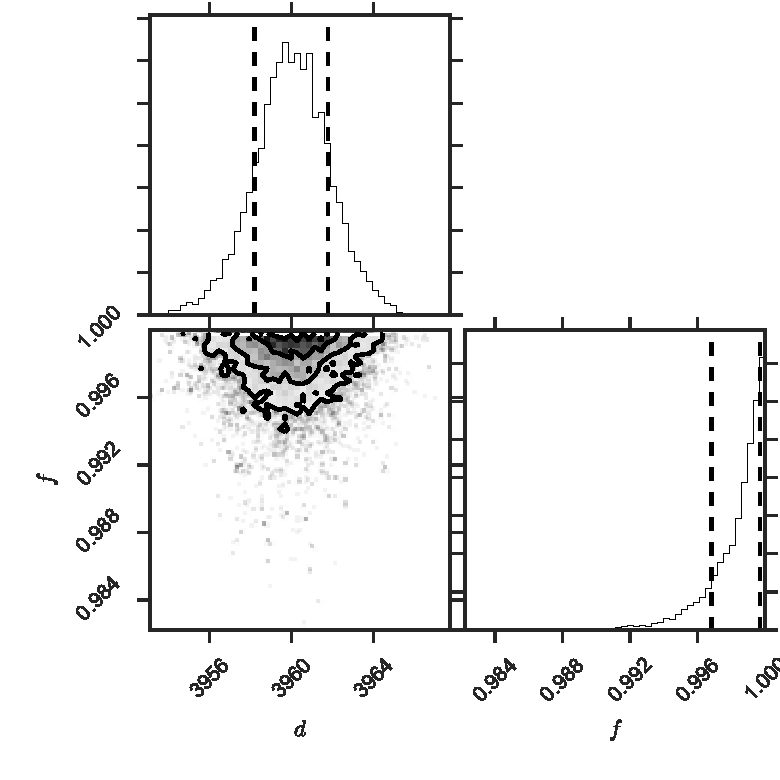
\includegraphics[width=\textwidth]{figs/VG03_corner.pdf}
              \caption{Fitted gap size $d$ and fill factor $f$ for VG03 hole region}
		\label{figVG03_corner}
        \end{subfigure}
	
        \begin{subfigure}[b]{0.5\textwidth}
                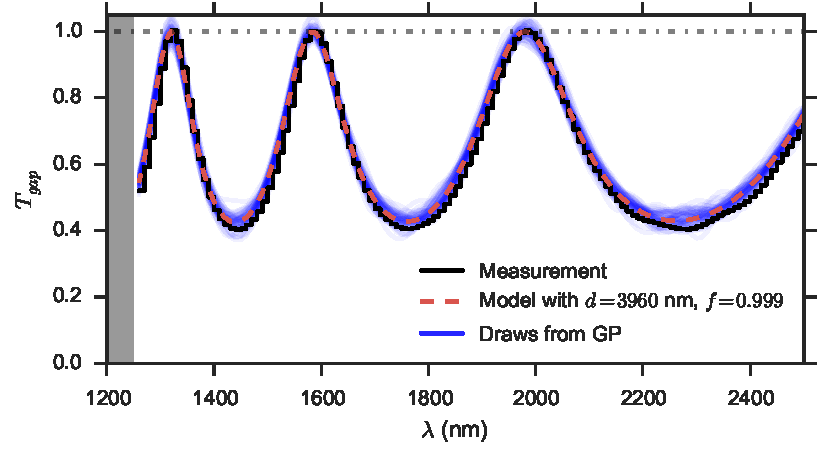
\includegraphics[width=\textwidth]{figs/VG03_f100.pdf}
                \caption{Measured spectrum and fit of VG03 hole region}
                \label{figVG03_f100}
        \end{subfigure}
\caption{ \emph{Top panel:} Corner plot of MCMC samples in our non-linear model fit of the transmission spectrum of Si optic part \# VG03.  The physical parameters of the model are the axial extent of the gap $d$, and the areal fill factor $f$ of the gap over the measurement region.  The MCMC model fit also includes nuisance parameters $a$ and $s$ (not shown) for the Gaussian Process covariance model.  \emph{Bottom panel:}Transmission through bonded Si sample VG03, normalized by the transmission of a DSP Si wafer. VG03 has a gap of axial extent $\sim4\;\mu$m implanted in its interface.  The measured spectrum (black stepped line) in this region shows characteristic Fabry-P\`erot fringes of constructive and destructive interference.  The only tunable parameters of the model are the gap axial extent, $d$ and fill factor $f$.  No scaling has been applied.  The red dashed line shows the best model fit with $d$ = 3960 $\pm$ 2 nm, consistent with 100\% fill factor.  The blue band shows the collective locations of 60 random draws from the Gaussian process model, described in the text.  Wavelengths shortward of 1250 nm (gray band) were not included in the fit, since Si is absorptive there.\label{figVG03full} }
\end{figure}


\begin{figure}[htbp]
        \centering
        \begin{subfigure}[b]{0.5\textwidth}
              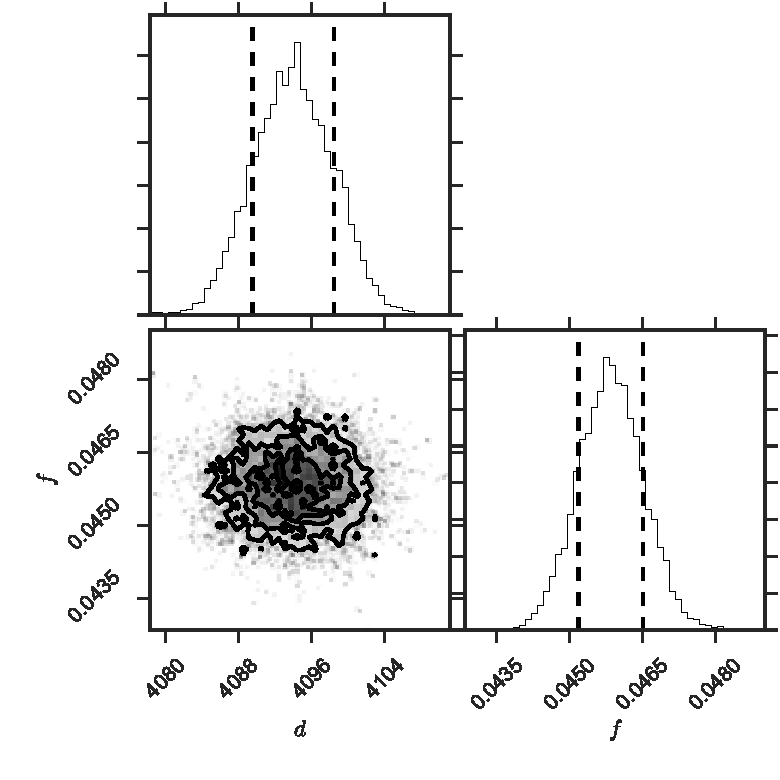
\includegraphics[width=\textwidth]{figs/VG03p2_corner.pdf}
              \caption{Fitted gap size $d$ and fill factor $f$ for VG03 petal region}
		\label{figVG03p2_corner}
        \end{subfigure}
	
        \begin{subfigure}[b]{0.5\textwidth}
                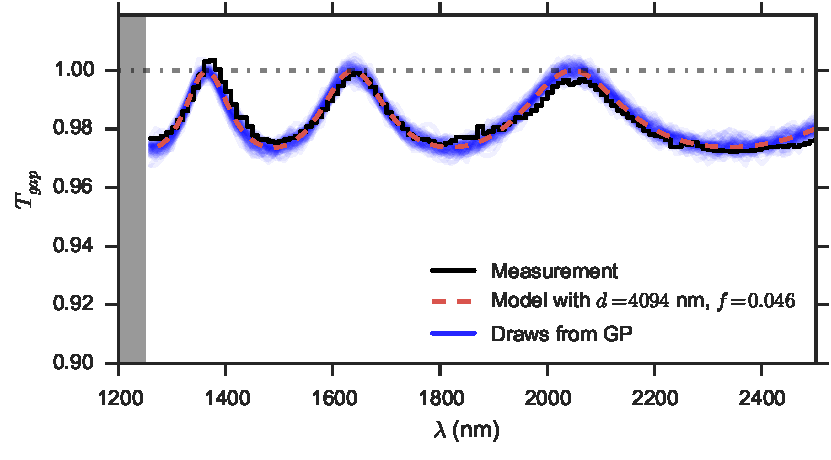
\includegraphics[width=\textwidth]{figs/VG03_f045.pdf}
                \caption{Measured spectrum and fit of VG03 petal region}
                \label{figVG03_f045}
        \end{subfigure}
\caption{ Same as Figure \ref{figVG03full}, but the measurement was in a region where less than $<5\%$ of the area exhibited the $\sim4\; \mu$m gap.  The measured spectrum in this region shows subdued Fabry-P\`erot fringes of constructive and destructive interference. The model derived axial extent is 4094 $\pm$ 5 nm covering a fill factor of 4.58 $\pm$ 0.06$\%$. \label{figVG03part}}
\end{figure}


\begin{figure}[htbp]
        \centering
        \begin{subfigure}[b]{0.5\textwidth}
              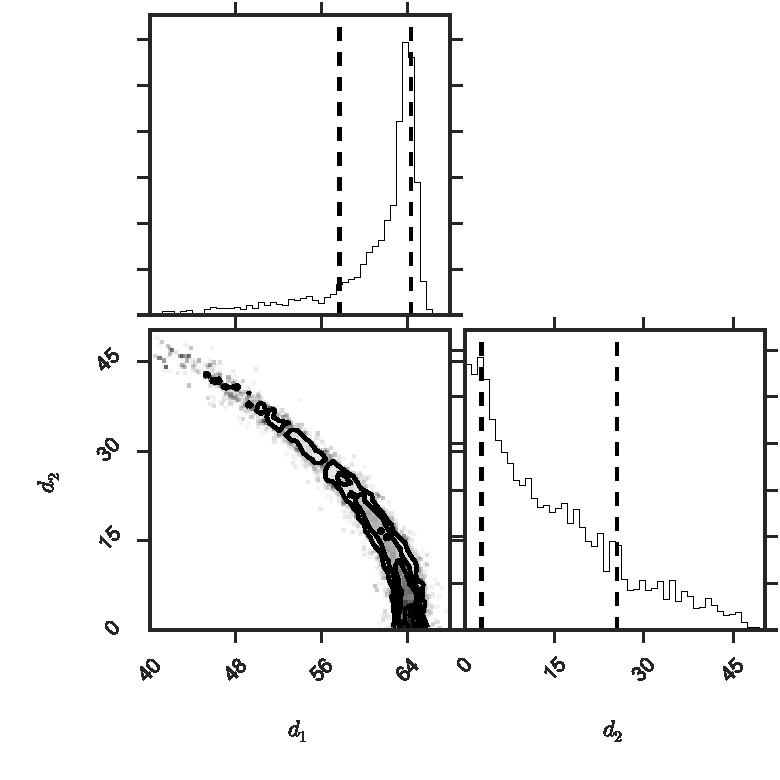
\includegraphics[width=\textwidth]{figs/VG12_twoGaps_corner.pdf}
              \caption{Fitted gap sizes $d_1$ and $d_2$ for VG09-12}
		\label{figVG12_corner}
        \end{subfigure}
	
        \begin{subfigure}[b]{0.5\textwidth}
                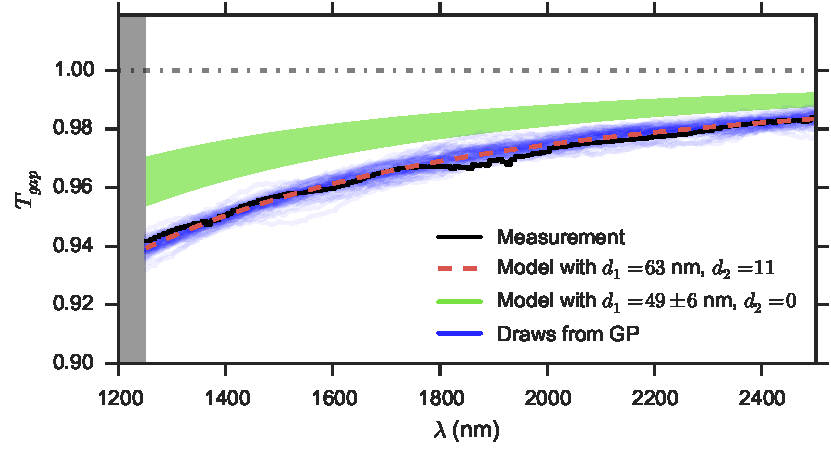
\includegraphics[width=\textwidth]{figs/VG12_twoGaps.pdf}
                \caption{Measured spectrum and fit of VG09-12}
                \label{figVG12_f50}
        \end{subfigure}
\caption{ Same as Figure \ref{figVG03full} and \ref{figVG03part}, but for sample VG09-12, which has an imbedded gap of axial extent $d=49\pm6\;$nm with fill factor $f=0.5$.  The measured spectrum in this region shows a clear deficit of transmission from the gapless counterparts.  The measured spectrum also shows a deficit of transmission compared to the predicted transmission of a 49 $\pm6\;$nm gap with 50\% fill factor (green apple shaded color band).  The discord between prediction and measurement could be due to several factors including an underestimate of the intrinsic gap size, an underestimate of the intrinsic fill factor, or an additional gap in excess of the prediction.  We favor the latter interpretation, since undesired gaps are common in these direct-bonded Si samples that have not undergone high-temperature thermal annealing.
\label{figVG12}}
\end{figure}

A key result of this work is to show that gaps of known dimensions are recovered in our spectroscopy.  Table \ref{tbl_DerivedGapSizes} summarizes the outcome of some measurements in the areas with known gaps and fill factors.  The table lists the median sample and 68\% confidence intervals.

\subsection{TODO: Comparison of Transmission-spectroscopy derived gap sizes with lab-measured gap size}


\subsection{TODO: Spectra of direct bonded Si with no intentionally implanted gaps}
\section{TODO: Discussion}

\subsection{TODO: Mitigation of measurement artifacts}
We mitigated measurement artifacts in the following ways.  We have mostly been able to rule out wavelength-dependent diffraction from the mesh pattern as a measurement artifact, since the beam size is large and the angular spread of diffraction from the mesh pattern would be much smaller than the spread of the beam.  Still, to remove this concern, we moved to using the coarse mesh rather than the medium or fine meshes, when possible.  We saw no difference in the bond quality surrounding the medium or fine meshes, which is consistent with results from the literature \cite{1992JEMat..21..669M}.  Specifically, the gas pressure of bonded wafers grows as the fill factor of gaps decreased.  In other words, what matters is the fill factor of gaps, not their relative sizes.  Since the fine, medium, and coarse meshes had the same fill factors, we anticipate no difference in the pressure of the gaps, and therefore no difference in the bonding properties.


\section{Conclusions}
We have described a measurement technique and laid out an analysis formalism for the detection and measurement of sub-wavelength gaps at Si-Si interfaces.  Experimental measurements show that we can precisely recover the extent of wavelength-scale gaps of known size, account for the presence of small gaps, and capture results consistent with no gap when measuring a monolithic part.

The technique and formalism we describe here can detect and measure the axial extent of gaps in Si-Si optical bonds down to a level of $20-30\;$nm.  It makes use of widely available off-the-shelf metrology equipment and simple to implement analysis.  Armed with this technique, optical fabricators have a new diagnostic tool to assess the quality of Si-Si bonds.

\appendix

\section{Incoherent Multiple Reflections Transfer Matrix Method}
\label{sec:Append-IMRTMM}

The wave transfer matrix method is described in detail in chapter 7 by Saleh and Teich in ``Fundamentals of Photonics'' \cite{2007fuph.book.....S}.  Briefly, their technique is to assemble a 2$\times$2 scattering matrix $\boldsymbol{S}$ which has the elements:
\begin{eqnarray}
\boldsymbol{S} = \left(
\begin{array}{cc}
 t_{12} & r_{21} \\
 r_{12} & t_{21} \\
\end{array}
\right)
\end{eqnarray}
Where $t$ and $r$ stand for transmission and reflection respectively.  The order of subscripts is the order of origin and destination of the wave in regards to the interface, so we know something about the direction of the wave and how it got there.  The $\boldsymbol{S}$ matrix encapsulates all the information we need to know about how light waves interact with the interface.  The real power of the matrix technique comes from a cousin of the scattering matrix, the so-called wave transfer matrix, $\boldsymbol{M}$.  The matrix $\boldsymbol{M}$ has the convenient property that its output can be used as the input for another matrix.  In other words, the input vector to $\boldsymbol{M}$ is made of the left and right moving components directly before the interface; the outputs are the left and right moving components directly after the interface:
\begin{eqnarray}
\left(
\begin{array}{c}
 U_2^{(+)} \\
 U_1^{(-)} \\
\end{array}
\right)=\boldsymbol{S} \left(
\begin{array}{c}
 U_1^{(+)} \\
 U_2^{(-)} \\
\end{array}
\right) \\
\left(
\begin{array}{c}
 U_2^{(+)} \\
 U_2^{(-)} \\
\end{array}
\right)=\boldsymbol{M} \left(
\begin{array}{c}
 U_1^{(+)} \\
 U_1^{(-)} \\
\end{array}
\right)
\end{eqnarray}

The elements of $\boldsymbol{S}$ and $\boldsymbol{M}$ are related to each other by geometric transformations\cite{2007fuph.book.....S}.  In thin films, the wavelength is comparable to the size of the dielectric layer and the vector components $U_{i}$ represent the complex amplitudes of the electromagnetic waves.  The polarization state can be encapsulated in scattering matrix components\cite{2007fuph.book.....S}.  The intensities of the emergent spectrum can be computed from the absolute square of the complex amplitudes.  For thick films, the vector components are the intensities of the emergent spectrum, since waves are incoherent.  \cite{2002ApOpt..41.3978K} work out the general transfer-matrix method for optical multilayer systems with incoherent interference.  The key idea for the incoherent transfer matrix method approach is to populate a scattering matrix with elements equal to the (wavelength dependent) transmitted $T_i$ and reflected $R_i$ intensities of an interface or set of interfaces that act together.  Then, use the geometric transformations to construct the $\boldsymbol{M}$ matrix.  

The matrix for the silicon air gap is calculated in the following way.  The first key idea is to treat the entire air gap as an abstraction, a Fabry-P\`erot etalon.  We do not need to bother to consider the microscopic coherent interactions with the etalon transmission, all of that information is encapsulated in these equations for a Fabry-P\`erot etalon:

\begin{eqnarray}
 \delta = \frac{2\pi}{\lambda}2d \label{eq:phase} \\
  F \equiv \frac{4R}{(1-R)^2} \\
 T_e = \frac{1}{1+F\sin^2(\delta/2)}  \label{eq:FabPerot}
\end{eqnarray}

with $\lambda$ the vacuum wavelength, $R$ the Fresnel reflection of silicon, and $F$ the coefficient of finesse.  The coefficient of finesse $F$ and the phase $\delta$ are the two parameters of the Fabry-P\`erot etalon.  The coefficient of Finesse encapsulates the Fresnel reflection and depends only on the Si refractive index which has only a small wavelength (and temperature) dependence.  The phase depends (Equation \ref{eq:phase}) on the wavelength $\lambda$ and $d$ the air gap spacing.  We assume the etalon is lossless, i.e. $T_e+R_e=1$.  So the incoherent scattering and transfer matrices for the etalon are:

\begin{eqnarray}
\boldsymbol{S_e}&=&\frac{1}{1+F\sin^2{\delta/2}} \left(
\begin{array}{cc}
1 & F \sin ^2(\delta/2) \\
F \sin ^2(\delta/2) & 1 \\
\end{array}
\right) \nonumber \\
\nonumber \\
\boldsymbol{M_e}&=&\left(
\begin{array}{cc}
 1-F \sin ^2(\delta/2) & F \sin ^2(\delta/2) \\
 -F \sin ^2(\delta/2) & 1+F \sin ^2(\delta/2) \\
\end{array}
\right)
\label{eqn:EtalonMatrix}
\end{eqnarray}

We assembled the matrix for the Air-Si Fresnel interface at the exterior of the bonded Si parts in the following way.  First it is important to note that the matrix is the same whether the transmission is from Si to air or air to Si.  This reciprocity is not necessarily true for the complex amplitudes matrix, but our approach employs intensities not complex amplitudes.  The Fresnel interface is lossless.  The transmission and reflection are given by the Fresnel equation for normal incidence:
\begin{eqnarray}
T_n&=&\frac{4n_{Si}}{(n_{Si}+1)^2} \\
R_n&=&\frac{(n_{Si}-1)^2}{(n_{Si}+1)^2} \label{eq:FresnelTrans}
\end{eqnarray}
For clarity I will drop the subscripts from $n_{Si}$, since we have already set $n_{air}=1$ and there are no other dielectric interfaces to think about.  So the scattering and transfer matrices for the air-Si Fresnel boundary are:

\begin{eqnarray}
\boldsymbol{S_n}&=&\frac{1}{(n+1)^2} \left(
\begin{array}{cc}
4n & (n-1)^2 \\
(n-1)^2 & 4n \\
\end{array}
\right)  \nonumber \\
\nonumber \\
\boldsymbol{M_n}&=&\frac{1}{4n}\left(
\begin{array}{cc}
 -n^2+6  n-1 & ( n-1)^2 \\
 -( n-1)^2 & ( n+1)^2 \\
\end{array}
\right)
\label{eqn:SiAirMatrix}
\end{eqnarray}

Finally, we cascade the matrices together to compute the net transmission through the stack of abstractions.  The result is a $2\times2$ transfer matrix: 

\begin{eqnarray}
\boldsymbol{M_{net}}=\boldsymbol{M_n}\boldsymbol{M_e}\boldsymbol{M_n}
\end{eqnarray}

From the matrix transformation equations \cite{2007fuph.book.....S} we know $M_{22}=1/T$.  Taking the inverse of the bottom right element of $\boldsymbol{M_{net}}$, we get the transmission $T_{net}$ through the net optical device: 

\begin{eqnarray}
T_{net}=\frac{2 n}{1+ 2n F\sin ^2(\delta/2)+n^2} \label{eqn:FPmatTrans}
\end{eqnarray}

Compare equations \ref{eqn:FPmatTrans} and \ref{eq:FabPerot}.  The revised transmission has picked up a few factors of 2 and $n$.  While we are at it, let's compute the matrix for the scenario with no intermediate etalon: there are simply two Fresnel interfaces with which light interacts incoherently.  This scenario is the model for a single DSP reference sample. The revised matrix multiplication is simply $\boldsymbol{M_{DSP}}=\boldsymbol{M_n}\boldsymbol{M_n}$.  Taking the inverse of the $M_{22}$ element, we find: 

\begin{eqnarray}
T_{DSP}=\frac{2 n}{n^2+1}\label{eqn:EqofSummedSlab}
\end{eqnarray}

which is identical to the result obtained by directly summing the intensities from multiple reflections:
\begin{eqnarray}
T_{DSP}=T^2 \sum_{i=0}^{N}R^{2i} \label{eqn:multsum}
\end{eqnarray}

It is informative to isolate the effect of the gap by dividing the measured bonded wafer transmission by the transmission of a reference DSP Si part.  We call this normalized transmission the etalon transmission $T_{e}$:
\begin{eqnarray}
T_{e} = T_{net}/T_{DSP} \\
T_{e} = \frac{n^2+1}{2 n F \sin ^2(\delta/2)+n^2+1} \label{eqn:Tetalon}
\end{eqnarray}


\bibliographystyle{osajnl}
\bibliography{AO_bondedSi}


%\begin{thebibliography}{99}

%% Do not include separate BibTeX files; if BibTeX is used,
%% paste the output (contents of .bbl file) here.

%\end{thebibliography}

\end{document}
